\documentclass[11pt,a4paper,onecolumn]{article}
\usepackage[utf8]{inputenc}
\usepackage{amsmath}
\usepackage{amsfonts}
\usepackage{amssymb}
\usepackage{graphicx}
\usepackage[dvipsnames]{xcolor}
\usepackage{cleveref}
\usepackage{pdflscape}
\usepackage{caption}
\usepackage{subcaption}
\usepackage{setspace}
\onehalfspacing


\usepackage[							% use biblatex for bibliography
	backend=bibtex,		% 	- use biber backend (bibtex replacement) or bibtex
	bibencoding=utf8,			% 	- use auto file encode
	style=authoryear-icomp,				% 	- use alphabetic (or numeric) bib style
	natbib=true,					% 	- allow natbib commands
	hyperref=true,					% 	- activate hyperref support
	backref=true,					% 	- activate backrefs		%TODO true in final
	isbn=false,						% 	- don't show isbn tags
	url=false,							% 	- don't show url tags
	doi=false,						% 	- don't show doi tags
	urldate=long,					% 	- display type for dates
	dashed=false,					%  - don't convert duplicate author names to dashes
	maxbibnames=100,%
	maxcitenames=2,%
]{biblatex}
	
\addbibresource{../../library.bib}
\addbibresource{../../Zimmerer2015.bib}


\newcommand{\TODO}[1]{{\color{red}\textbf{[TODO #1]}}}

\DeclareGraphicsExtensions{.pdf,.png}


\title{{\large \textit{Summary of the M.Sc. thesis:}}\\
\textbf{Automatic diagnosis and feedback for\\lexical stress errors in non-native speech}\\
{\Large Towards a CAPT system for French learners of German}}

\date{}

\begin{document}
\maketitle

\section{Introduction}

The prosodic realization of lexical stress, the phenomenon by which certain syllable(s) in a word are accentuated more than others, is an important feature of the German phonological system, and may have a large impact on the intelligibility of non-native German speech \citep{Hirschfeld1994}. However, lexical stress can pose a considerable challenge to students learning German as a foreign language (L2), especially students whose native language (L1) is French \citep{Hirschfeld2007}. This thesis investigates how Computer Assisted Pronunciation Training (CAPT) can help L1 French speakers improve their lexical stress prosody in German. It describes the manual annotation of lexical stress errors in a small learner speech corpus, investigates a variety of methods for automatically diagnosing such errors in learner word utterances, and explores how these diagnoses can be used to deliver diverse types of feedback to learners.  Its most important contribution is a prototype CAPT tool called
\textbf{de-stress}: the German (\textbf{de}) \textbf{S}ystem for \textbf{T}raining and \textbf{R}esearch on \textbf{E}rrors in \textbf{S}econd-language \textbf{S}tress.\footnote{\texttt{github.com/vakila/de-stress}} 
%
This tool integrates various diagnostic and feedback methods via an easy-to-use web interface (see \cref{fig:interface}), and is designed not only to provide students with automatic, individualized feedback on their lexical stress errors, but also to facilitate future research on the efficacy of 
%the different 
various
diagnostic and feedback approaches. % explored in this thesis.



\section{Lexical stress errors by French learners \mbox{of German}}
\label{sec:lexstress}

In an effort to shed light on the nature of lexical stress errors in the speech of L1 French learners of German as L2, 
%\TODO{this chapter has described} original efforts to 
	%annotate and analyze such errors in a small corpus of learner speech.
	%
	%\TODO{As described in \cref{sec:lexstress:data,sec:lexstress:annotators,sec:lexstress:method},}
	lexical stress realizations in utterances of bisyllabic, initial-stress words %\TODO{(\cref{sec:lexstress:data})}
	taken from the IFCASL corpus (\cite{Trouvain2013,Fauth2014}) %; \TODO{see also \cref{sec:intro:ifcasl}) }
	were annotated by native and non-native German annotators with various levels of phonetics/phonology expertise. % with different L1s and phonetic training backgrounds \TODO{(\cref{sec:lexstress:annotators})}.
	%
	Annotators %used a graphical annotation tool to label each recorded 
	labeled each word utterance
	as correctly or incorrectly realizing lexical stress (i.e. the speaker clearly stressed the correct or incorrect syllable), failing to clearly realize stress (i.e. the speaker did not seem to stress either syllable), or having technical or other problems which prevented the assessment of lexical stress.  % \TODO{(\cref{sec:lexstress:method})}.
	
	Analysis of the labels assigned by different annotators to the same utterances %\TODO{(\cref{sec:lexstress:agreement})} 
	revealed relatively low inter-annotator agreement; % (see \TODO{TABLE}); %was \TODO{NUMBERS 
	%relatively low, with 
	%only ``fair'' %agreement 
	%\citep{Landis1977},} on average, between 
	on average, pairs of annotators who labeled the same utterances agreed on 54.92\% of utterances, and exhibited an average \citeauthor{Cohen1960}'s (\citeyear{Cohen1960}) Kappa ($\kappa$) value of 0.23.
	Considerable variation was observed among individual annotators, %\TODO{(\cref{sec:agreement:overall})}, 
	which did not seem to be explained by differences 
	in their L1 %\TODO{(\cref{sec:agreement:native})} 
	or level of phonetics/phonology expertise. %\TODO{(\cref{sec:agreement:expert})}. 
%	However, it was observed that
%	L2 German speakers annotated a higher proportion of utterances as having unclear stress compared to L1 speakers \TODO{(\cref{sec:agreement:native})}, and that expert annotators judged substantially higher proportion of utterances as correctly realizing stress compared to intermediate or novice annotators \TODO{(\cref{sec:agreement:expert})}.
%	\TODO{As described in \cref{sec:agreement:overall},} t
%	\TODO{remove?} 
%	There also seemed to be variability in inter-annotator 
%	agreement with respect to the different word types %represented 
%	in the dataset, and further work is needed to discern the factors responsible for this observation. % \TODO{(see \cref{sec:conclusion:future})}. 
	
	The multiple, often conflicting, error annotations from different annotators were consolidated into a single gold-standard annotation for each utterance in the dataset, %\TODO{(see \cref{sec:agreement:gold})}, 
	which served as the basis for an analysis of the frequency and type of errors produced by learners. % \TODO{(\cref{sec:lexstress:results})}. 
	%
	Overall, approximately two-thirds (63.77\%) of learners' utterances were deemed to realize lexical stress correctly, confirming that French learners of German frequently make errors with respect to lexical stress. %\TODO{(see \cref{sec:stress:expected,sec:targeting:frequency})}.
	%
	%\TODO{FIGURE(S)?}	
	The observed frequency of such errors was considerably lower in the speech of advanced learners than that of beginners, %\TODO{(\cref{sec:results:level})}, 
	and children (ages 15-16) seemed to make more errors than adult beginners; % \TODO{(\cref{sec:results:agegender})}; 
	no substantial difference was observed between speakers of different genders. 
%	As in the case of inter-annotator agreement, considerable variation was observed in the frequency of errors in utterances of different word types, % \TODO{(\cref{sec:results:wordtype})}, 
%	though once again the factors underlying this variability are not immediately evident and should be investigated in future work. % \TODO{\TODO{(see \cref{sec:conclusion:future})}}.
	
	The error annotation and analysis described in this chapter thus contribute considerably to our understanding of the difficulties L1 French speakers may have realizing lexical stress in 
	German, 
	and the fact that learners, especially beginners and children, seem to struggle with lexical stress production justifies the selection of lexical stress errors as the focus of this thesis project. Additionally, the analysis of inter-annotator agreement presented in this chapter, specifically the finding that the observed agreement was generally rather low,
	constitutes an important discovery with respect to the task of identifying such errors in learner speech:
	though further research is needed to determine why and under which conditions this is the case, % \TODO{(see \cref{sec:conclusion:future})}, 
	it would seem that diagnosing lexical stress errors may be a challenging task for at least some L1 and L2 German speakers. If true, this has important implications for the development and evaluation of automatic error diagnosis systems, 
	which is the subject of the following section.
	%which will be discussed further in \cref{sec:diag}.

\section{Diagnosis of lexical stress errors}
\label{sec:diag}

With the motivation of helping French learners of German correct these frequently-produced lexical stress errors, this thesis explores the methods by which such errors can be automatically diagnosed in learner speech. 
%
All diagnosis starts from a prosodic analysis of the learner's utterance in terms of duration, fundamental frequency (F0), and intensity, i.e. the three acoustic properties most strongly correlated with the prosodic realization of lexical stress (see e.g. \cite{Dogil1999,Cutler2005}), and whose perceptual correlates are timing, pitch, and loudness, respectively. %based on a segmentation of that utterance produced automatically by forced alignment. In the current implementation, de-stress mocks the alignment step by using pre-existing, automatically-produced segmentations for the utterances from the IFCASL corpus \citep{Fauth2014). 
This analysis requires reasonably accurate automatically-produced segmentations of the words, syllables, and phones of a given utterance; while forced alignment can theoretically be used to produce such segmentations on the fly when the text of the utterance is known \citep[e.g.]{Mesbahi2011}, the current implementation of de-stress mocks the alignment step by using pre-existing automatic segmentations for the utterances from the IFCASL corpus \citep{Fauth2014}.
Using these segmentations, features capturing the relative duration, F0, and intensity of each syllable in a given word utterance are automatically extracted using the speech processing functionality of the JSnoori software\footnote{\texttt{jsnoori.loria.fr}} \citep{Laprie1999,DiMartino1999}.

%This thesis explores methods by which lexical stress errors in the speech of French learners of German can be automatically diagnosed, as implemented in the modular diagnostic component of the de-stress CAPT tool.
	
	
	%The first requirement for error diagnosis, accurate automatically-produced segmentations of the words, syllables, and phones of a learner's utterance (or that of a native speaker), can be obtained through forced alignment with the text of the utterance, \TODO{as described in \cref{sec:diag:segmentation}}. Forced alignment for German utterances being currently under development in the JSnoori software used by de-stress for speech processing, the current version of de-stress mocks this alignment step by using automatically-produced segmentations for utterances from the IFCASL corpus (\cite{Fauth2014,Trouvain2013};\TODO{ see also \cref{sec:intro:ifcasl})}.
	
	%Analysis of the lexical stress realization of a given utterance, based on a set of prosodic features, is a second requirement for diagnosis, and \TODO{\cref{sec:diag:prosody} has presented }the set of features which can be used for such analysis in de-stress. These features capture the three acoustic properties most strongly correlated with the prosodic realization of lexical stress, namely duration, F0, and intensity. In de-stress, such features are extracted from a given utterance using the forced-alignment segmentations of that utterance and the speech processing capabilities of JSnoori.
	
	Using these features to represent a given learner's (L2) utterance as well as corresponding utterance(s) by L1 speakers, it is possible to assess the learner's utterance via one of two primary strategies: comparison or classification. 
	%\TODO{\Cref{sec:diag:compare} has explored} the possibilities for comparison-based diagnosis, in which 
	Diagnosis by comparison is the method most commonly used in past CAPT systems and research (see e.g. \cite{Eskenazi2009,Bonneau2011,Delmonte2011}).
	In the simplest comparison-based approach implemented in de-stress, features of the relevant segments of a learner's utterance are compared to the analogous features in a single L1 (reference) utterance using JSnoori, and an error is diagnosed when the utterances differ considerably with respect to the relevant features. 
	%\TODO{As described in \cref{sec:compare:single}}, JSnoori uses this comparison-based approach to score each L2 utterance with respect to duration, F0, and prosody, and de-stress can use these scores as one form of diagnosis and a starting point for the delivery of certain types of feedback, as will be discussed in\TODO{ \cref{chap:feedback}}. 
	%In addition to diagnosing an L2 utterance in comparison with a single L1 utterance, de-stress can combine scores with respect to multiple L1 utterances into a single score \TODO{(see \cref{sec:compare:multi})}, 
	To reduce some of the risk of the diagnosis ``over-fitting'' to speaker- or utterance-dependent features of a single reference, de-stress can average the results of multiple one-on-one comparisons to produce a multiple-reference diagnosis; this is a relatively novel approach to comparison-based diagnosis.
	Another innovation of de-stress relates to the method of choosing the reference utterance(s) for a given learner utterance; though most existing CAPT systems 
	%, including JSnoori, 
	require manual selection of reference utterances, previous research by \textcite{Probst2002} suggests that using an intelligently-selected reference speaker can help learners improve their pronunciation. Therefore, de-stress also offers an automatic selection option in which the reference is selected by choosing the L1 speaker(s) whose voice most closely resembles that of the learner, in terms of F0 mean and range.
	
	The second diagnosis strategy explored in this thesis, classification of errors using machine learning algorithms, is a more novel approach to lexical stress error identification in CAPT, in which a learner's utterance is compared to the more abstract model of L1 speech represented by a classifier trained on a large number of L1 utterances. Although some work has been done on classifying lexical stress patterns in English \citep{Shahin2012a,Kim2011}, the classification experiments conducted in this work %\TODO{described in \cref{sec:classification:features,sec:classification:unseen}} 
	constitute %original contributions to the understanding 
	the first known exploration of how, and how effectively, classification-based diagnosis can be used to identify (in)correct realizations of lexical stress in German. 
	%\TODO{As described in \cref{sec:classification:features}}, 
	Experiments with different prosodic feature sets 
	%(see \TODO{TABLE}) 
	suggest that the features seemingly most useful for classification relate to the duration and F0 of the utterance(s), unsurprising considering that these have been shown to be most closely linked to lexical stress in German \citep{Cutler2005,Dogil1999}. Features capturing the word type of the utterance as well as the age, gender and proficiency level of the speaker were also found to be quite valuable for error classification; combining these features with all three prosodic feature types resulted in the highest overall accuracy observed on this dataset (71.87\% accuracy, $\kappa=$ 0.34). As the observed agreement between the classifier's labels and the gold standard thus slightly exceeded the overall inter-annotator agreement observed when humans were asked to perform this error diagnosis task (see \cref{sec:lexstress}), these results seem encouraging. Unsurprisingly, slightly lower accuracy was observed when classifying utterances of word types or speakers not represented in the training data; however, the fact that accuracy on unseen words still remained comparable to the human inter-annotator agreement statistics seems to confirm the expectation that classification-based diagnosis may be a useful way to create CAPT systems which are are not limited to words/sentences for which recorded L1 utterances are available.
	
	
	%While comparison-based diagnosis is not a new approach to identifying lexical stress errors in CAPT, the availability of multiple-reference comparison and automatic selection of reference speakers in the system, as well as the ability for researchers or instructors to configure the comparison method, make de-stress an important addition to the current CAPT landscape. The inclusion of a classification-based alternative to diagnosis is also a novelty for such a CAPT system, and this chapter's investigation of how L2 lexical stress errors can be diagnosed by classification is one of the major contributions of this thesis. 
	In the administrative interface to de-stress (see \cref{fig:admin}), a researcher or instructor can choose between these various approaches for diagnosing lexical stress errors (see \cref{fig:createDM}).
	%By enabling researchers and instructors to choose among the various diagnosis options described in this chapter, 
	This modularity and flexibility enables de-stress to facilitate much needed future research  exploring which diagnostic methods are most useful to which learners in which situations. %, and which types of feedback %\TODO{(described in the following chapter)} can best convey these diagnoses to the learner.

\section{Feedback on lexical stress errors}

%\TODO{This chapter has presented} the diverse array of feedback methods offered by de-stress. 
Based on a diagnosis of the learner's lexical stress error(s) via one of the methods described in the previous section, the CAPT tool developed in this work can automatically generate and present explicit %\TODO{(\cref{sec:fb:explicit})} 
and/or implicit %\TODO{(\cref{sec:fb:implicit})} 
feedback on these errors. 
%
%Implicit feedback may be delivered visually, % \TODO{(\cref{sec:implicit:visual})}, 
%in the form of graphical  or textual representations of prosody which may be easier to interpret than the more direct representations of speech signals more frequently seen in CAPT systems, % \TODO{(see \cref{sec:bkgd:capt})}, 
%or via the auditory channel %\TODO{(\cref{sec:implicit:auditory})} 
%in the form of original or prosodically modified utterances. 
As seen in \cref{fig:interface}, implicit feedback may be delivered in the form of graphical abstractions of the prosodic features of each syllable in a given utterance, or via text stylization that uses font size to convey the most important acoustic correlate of lexical stress prosody, duration.
%
Explicit feedback options include graphical ``skill bars'' %\TODO{(\cref{sec:explicit:skillbars})} 
informing learners of the correctness of their pronunciation with regard to duration (timing), F0 (pitch), and intensity (loudness), as well as verbal feedback on this information via a series of error/success messages (see \cref{fig:explicitFB}). % \TODO{(\cref{sec:explicit:verbal})}. 
Finally, as self-assessment is a valuable way for learners to give themselves feedback on their own performance and take autonomous control of their learning \citep{Neri2002,Mehlhorn2005}, an additional feedback option offers learners the opportunity to self-assess their pronunciation via a short questionnaire. % \TODO{(\cref{sec:fb:selfassess})}, in the hopes of encouraging them to develop a metacognitive understanding of their own learning process and take autonomous control of their learning.


Thanks to its modular implementation of the various feedback types, in combination with a simple configuration interface that allows researchers and/or instructors to easily pick and choose from the available options (see \cref{fig:createFM}), %\TODO{(\cref{sec:fb:system})}, 
de-stress is therefore a valuable platform for future empirical investigations into the impacts of these feedback types on the 
acquisition of L2 word prosody 
by L1 French learners of German. 
%As established in \TODO{\cref{chap:background}} and further discussed in the following chapter, 
Much work remains to be done to determine which feedback types are most effective in which learning contexts; by presenting a tool to facilitate such research, ostensibly the first of its kind for this type of error and aimed at this group of learners, this thesis has thus made an important contribution towards a more detailed understanding of the relative efficacy of feedback types in CAPT.


\section{Conclusion}

This thesis thus presents original work taking steps towards the development of a comprehensive, intelligent CAPT system for French learners of German. Drawing from previous research on foreign-language pedagogy, phonetics/phonology, and speech technology, as well as original research on the frequency of lexical stress errors in learner speech and novel methods for diagnosing such errors, the de-stress system developed in this thesis project is the first known CAPT tool dedicated to helping L1 French speakers improve their realization of lexical stress in German, and to facilitating research on the use of automatic, individualized feedback to help learners correct such errors. 
Once more is known about which diagnosis and feedback methods should be used in which contexts, this tool could become a useful component of a fully-fledged intelligent CAPT system, in which
models of relevant aspects of the learning context (e.g. the student's skill level, progress, or personal preferences)
are used to automatically decide which modules of the tool to activate. %, as \TODO{\cref{fig:hourglass-ITS}} illustrates.
%\TODO{SOMETHING ABOUT INTEGRATION WITH ITS - The following section suggests some possible directions for future work on improving de-stress and using it to make further advancements in CAPT for German.}



\clearpage



%%% FIGURES

% Student interface
		\begin{figure}[p]
		\makebox[\textwidth][c]{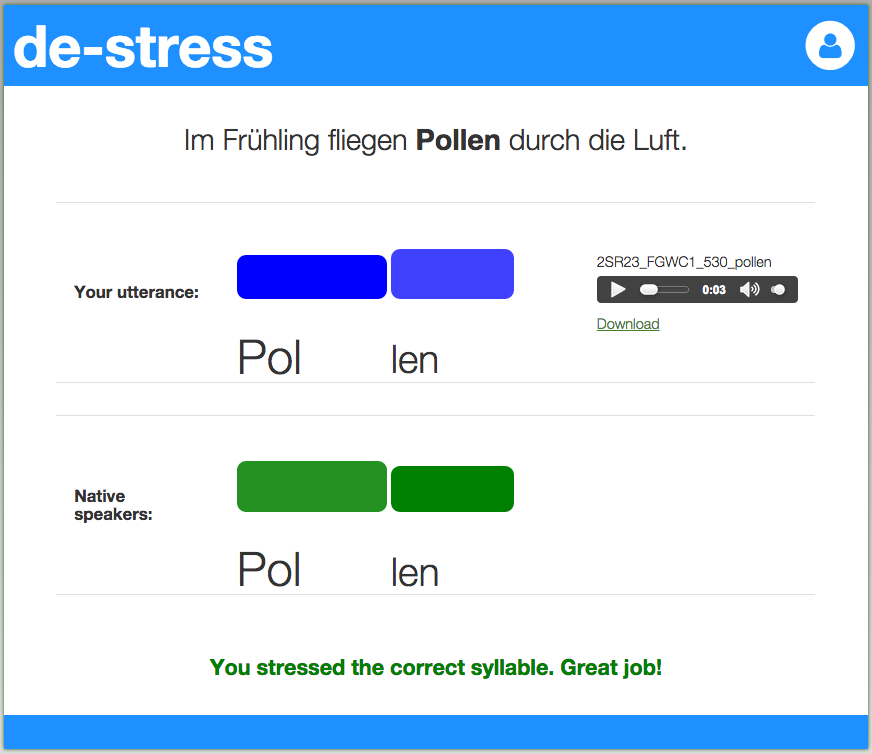
\includegraphics[width=1.3\textwidth]{../../img/screenshots/StudentInterface-userIcon}}
		\caption{Screenshot of feedback delivery in the student-facing web interface of the prototype CAPT tool de-stress.
		The implicit feedback options depicted include graphical abstractions of prosody (the width, height, and opacity of each colored rectangle visualize the relative duration, mean F0, and mean intensity of the corresponding syllable)
		and text stylization (font size corresponds to duration).
		}
		\label{fig:interface}
		\end{figure}
		
%\begin{landscape}
%	\begin{figure}
%	\centering
% Implicit FB
%		%\begin{subfigure}[b]{.3\paperheight}
%		\begin{figure}
%		\centering
%		\makebox[\textwidth][c]{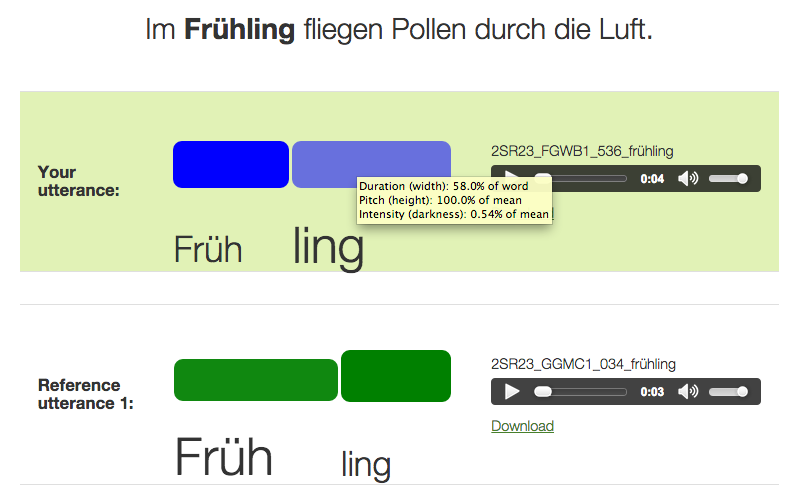
\includegraphics[width=1.3\textwidth]{../../img/screenshots/rectanglesWithOpacity}}
%		\caption{Implicit feedback options,
%		%The sentence at the top shows the target word (``Fr\"{u}hling'') in bold. 
%		including graphical abstractions of prosody (the width, height, and opacity of each colored rectangle visualize the relative duration, mean F0, and mean intensity of the corresponding syllable, with the yellow tooltip text displaying exact values when the mouse hovers over a rectangle)
%		and text stylization (font size corresponds to duration).
%		%The duration, mean F0, and mean intensity of each syllable of the learner and reference utterances are visualized respectively by the width, height, and opacity of the corresponding colored rectangle, with precise values for each of the three features visible in the yellow tooltip box which appears when the learner hovers the mouse over a given rectangle. The font size of the syllable's text visualizes the duration of that syllable. 
%		%Learners may listen to each utterance using the controls on the right.
%		}
%		\label{fig:implicitFB}
%		\end{figure}	

% Explicit FB
		%\begin{subfigure}[b]{.3\paperheight}
		\begin{figure}
		\centering
		\makebox[\textwidth][c]{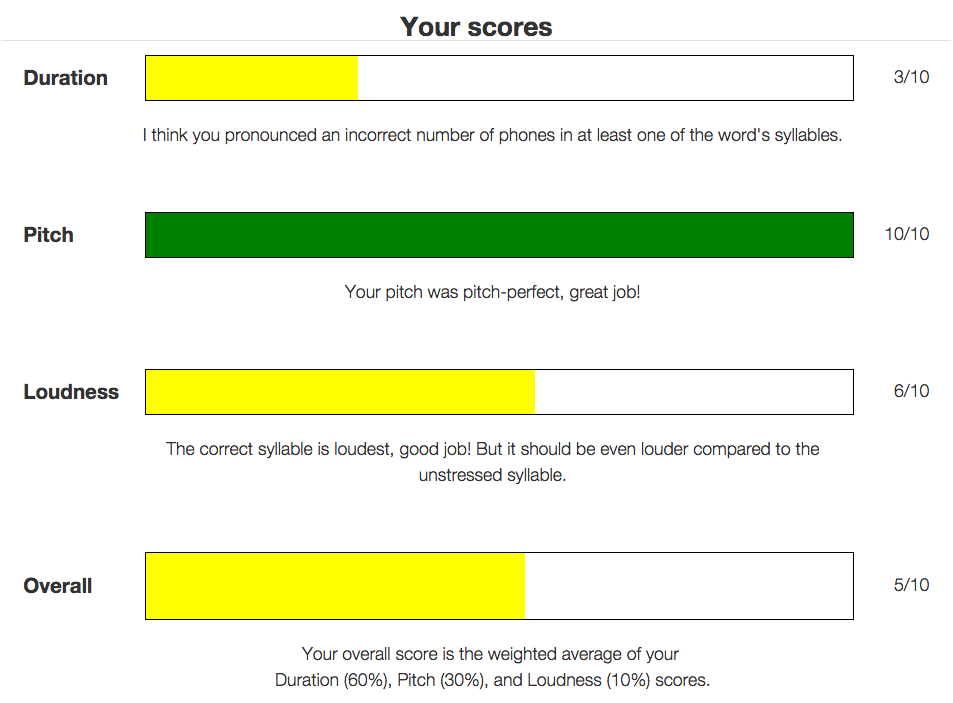
\includegraphics[width=1.3\textwidth]{../../colloquium/SkillBarsWithMessages}}
		\caption{Explicit feedback options, including feedback via ``skill bars'' and via verbal error/success messages.}
		\label{fig:explicitFB}
		\end{figure}
%	\end{figure}
%\end{landscape}		
		
% Teacher interface
		\begin{figure}
		\makebox[\textwidth][c]{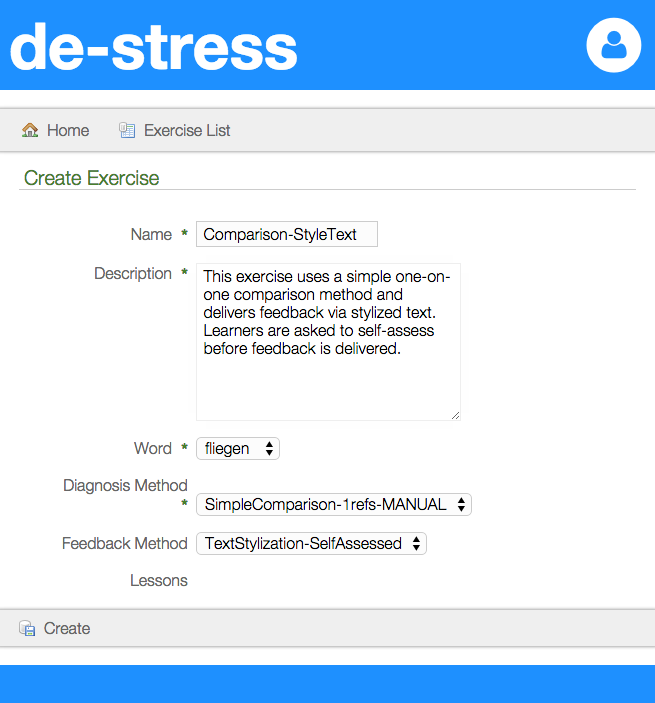
\includegraphics[width=1.3\textwidth]{../../img/screenshots/TeacherInterface-smaller}}
		\caption{Screenshot of the administrative interface allowing a researcher or instructor to create an exercise utilizing certain diagnosis and feedback options (see \cref{fig:createDM,fig:createFM}).}
		\label{fig:admin}
		\end{figure}

% Create DM

	\begin{figure}
	\centering
	\includegraphics[width=.7\textwidth]{../../colloquium/createDM} 
	\caption{Administrative interface for selecting diagnosis options.}
	\label{fig:createDM}
	\end{figure}

%	\begin{figure}
%		\centering
%		%\makebox[\textwidth][c]{%
%%			\begin{tabular}{p{0.5\textwidth} p{0.5\textwidth}}
%%			  \vspace{0pt} 
%			  \includegraphics[width=.7\textwidth]{../../colloquium/createDM} %&
%			 % ~
%%			  \vspace{0pt} 
%			  \includegraphics[width=.7\textwidth]{../../colloquium/createFM}
%%		\end{tabular}
%		%}
%	\end{figure}

% Create FM

	\begin{figure}
	\centering
	\includegraphics[width=.7\textwidth]{../../colloquium/createFM} 
	\caption{Administrative interface for selecting feedback options.}
	\label{fig:createFM}
	\end{figure}

\clearpage
\printbibliography[title={References}]

\end{document}